\documentclass{beamer}
\usetheme{default}
\usepackage[italian]{babel}
%\usepackage{t1enc}
\usepackage{pgfpages}
\usepackage{listings}
%\pgfpagelayout{2 on 1}[a4paper]

%\usepackage{../../common/espacs}
\lstset
{
  language=[ISO]C++,                       % The default language
  basicstyle=\sf,                          % The basic style
  keywordstyle=\color{blue}\bfseries,      % Set keyword style
  commentstyle=\color{darkgreen}\itshape,  % Set comment style
  extendedchars=true                       % Allow extended characters
}

\setbeamercovered{transparent}

\begin{document}

%---------------------------------------------------------------------------------

\begin{frame}[fragile]

    Short introduction to Eclipse

\end{frame}

%---------------------------------------------------------------------------------

\begin{frame}[fragile]

    \frametitle{Eclipse}

    Get Eclipse on the website

    \begin{verbatim}
        http://www.eclipse.org/downloads/
    \end{verbatim}

    Get the package

    \begin{figure}
        \centering
        
\includegraphics[width=0.5\textwidth]{./images/eclipselogo}
    \end{figure}

    Unpack it and run eclipse

\end{frame}

%---------------------------------------------------------------------------------

\begin{frame}[fragile]

    \frametitle{Eclipse: create a new project}

    \begin{figure}
        \centering
        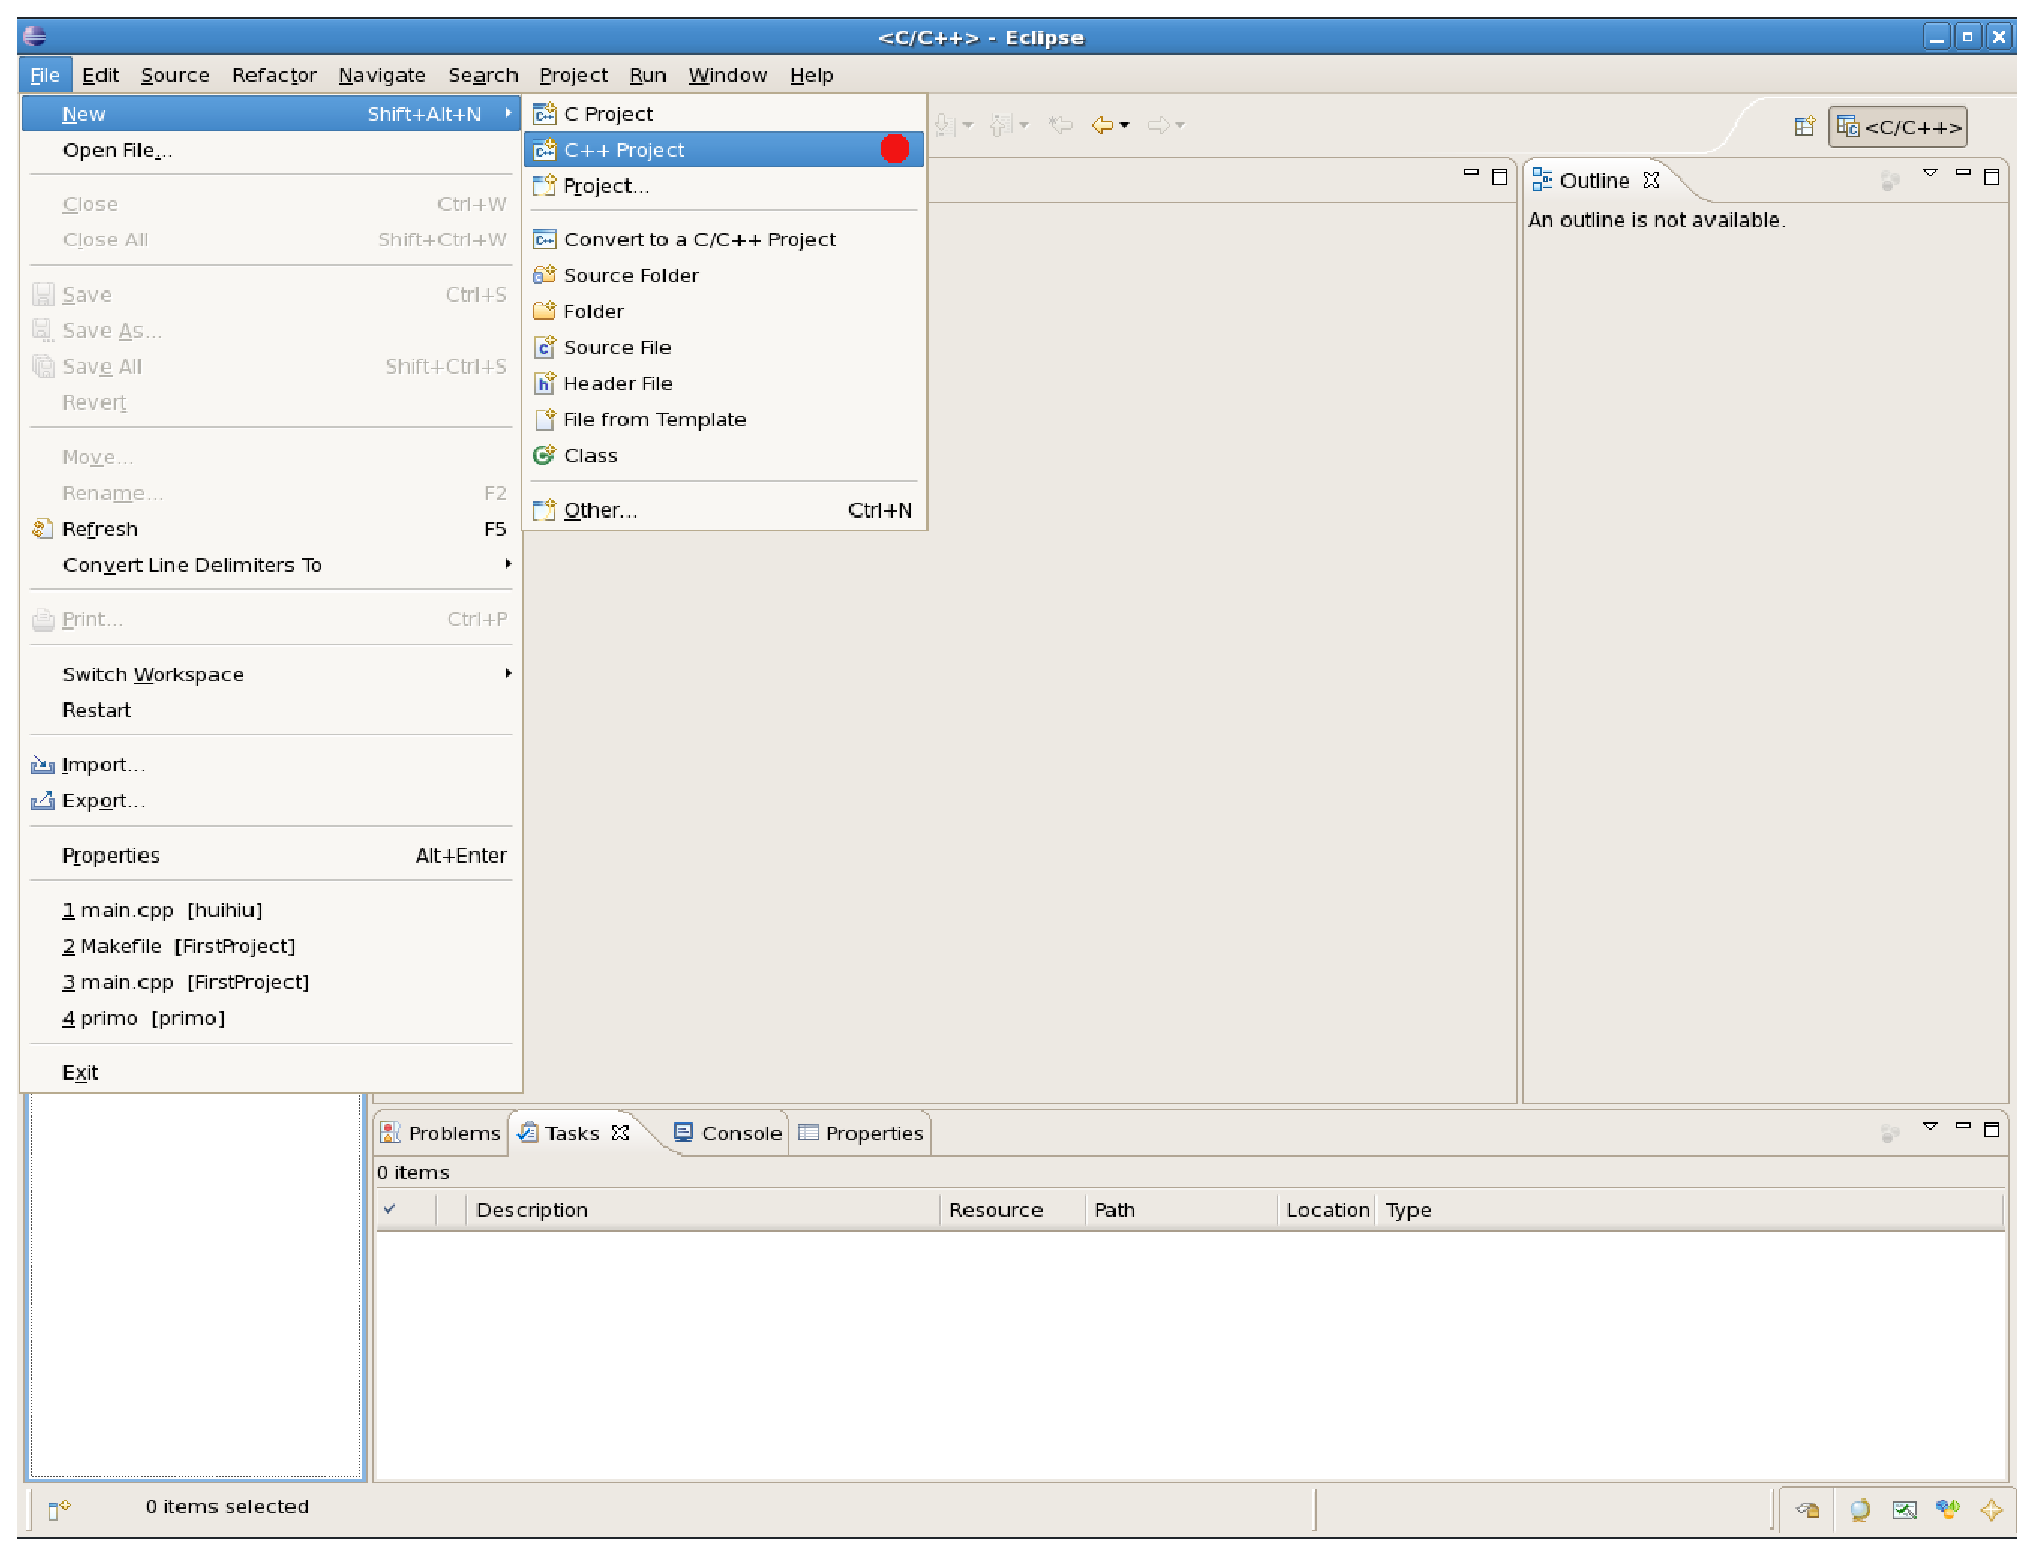
\includegraphics[width=0.95\textwidth]{./images/eclipse1}
    \end{figure}

\end{frame}

%---------------------------------------------------------------------------------

\begin{frame}[fragile]

    \frametitle{Eclipse: insert name, compiler and select without automatico Makefile}

    \begin{figure}
        \centering
        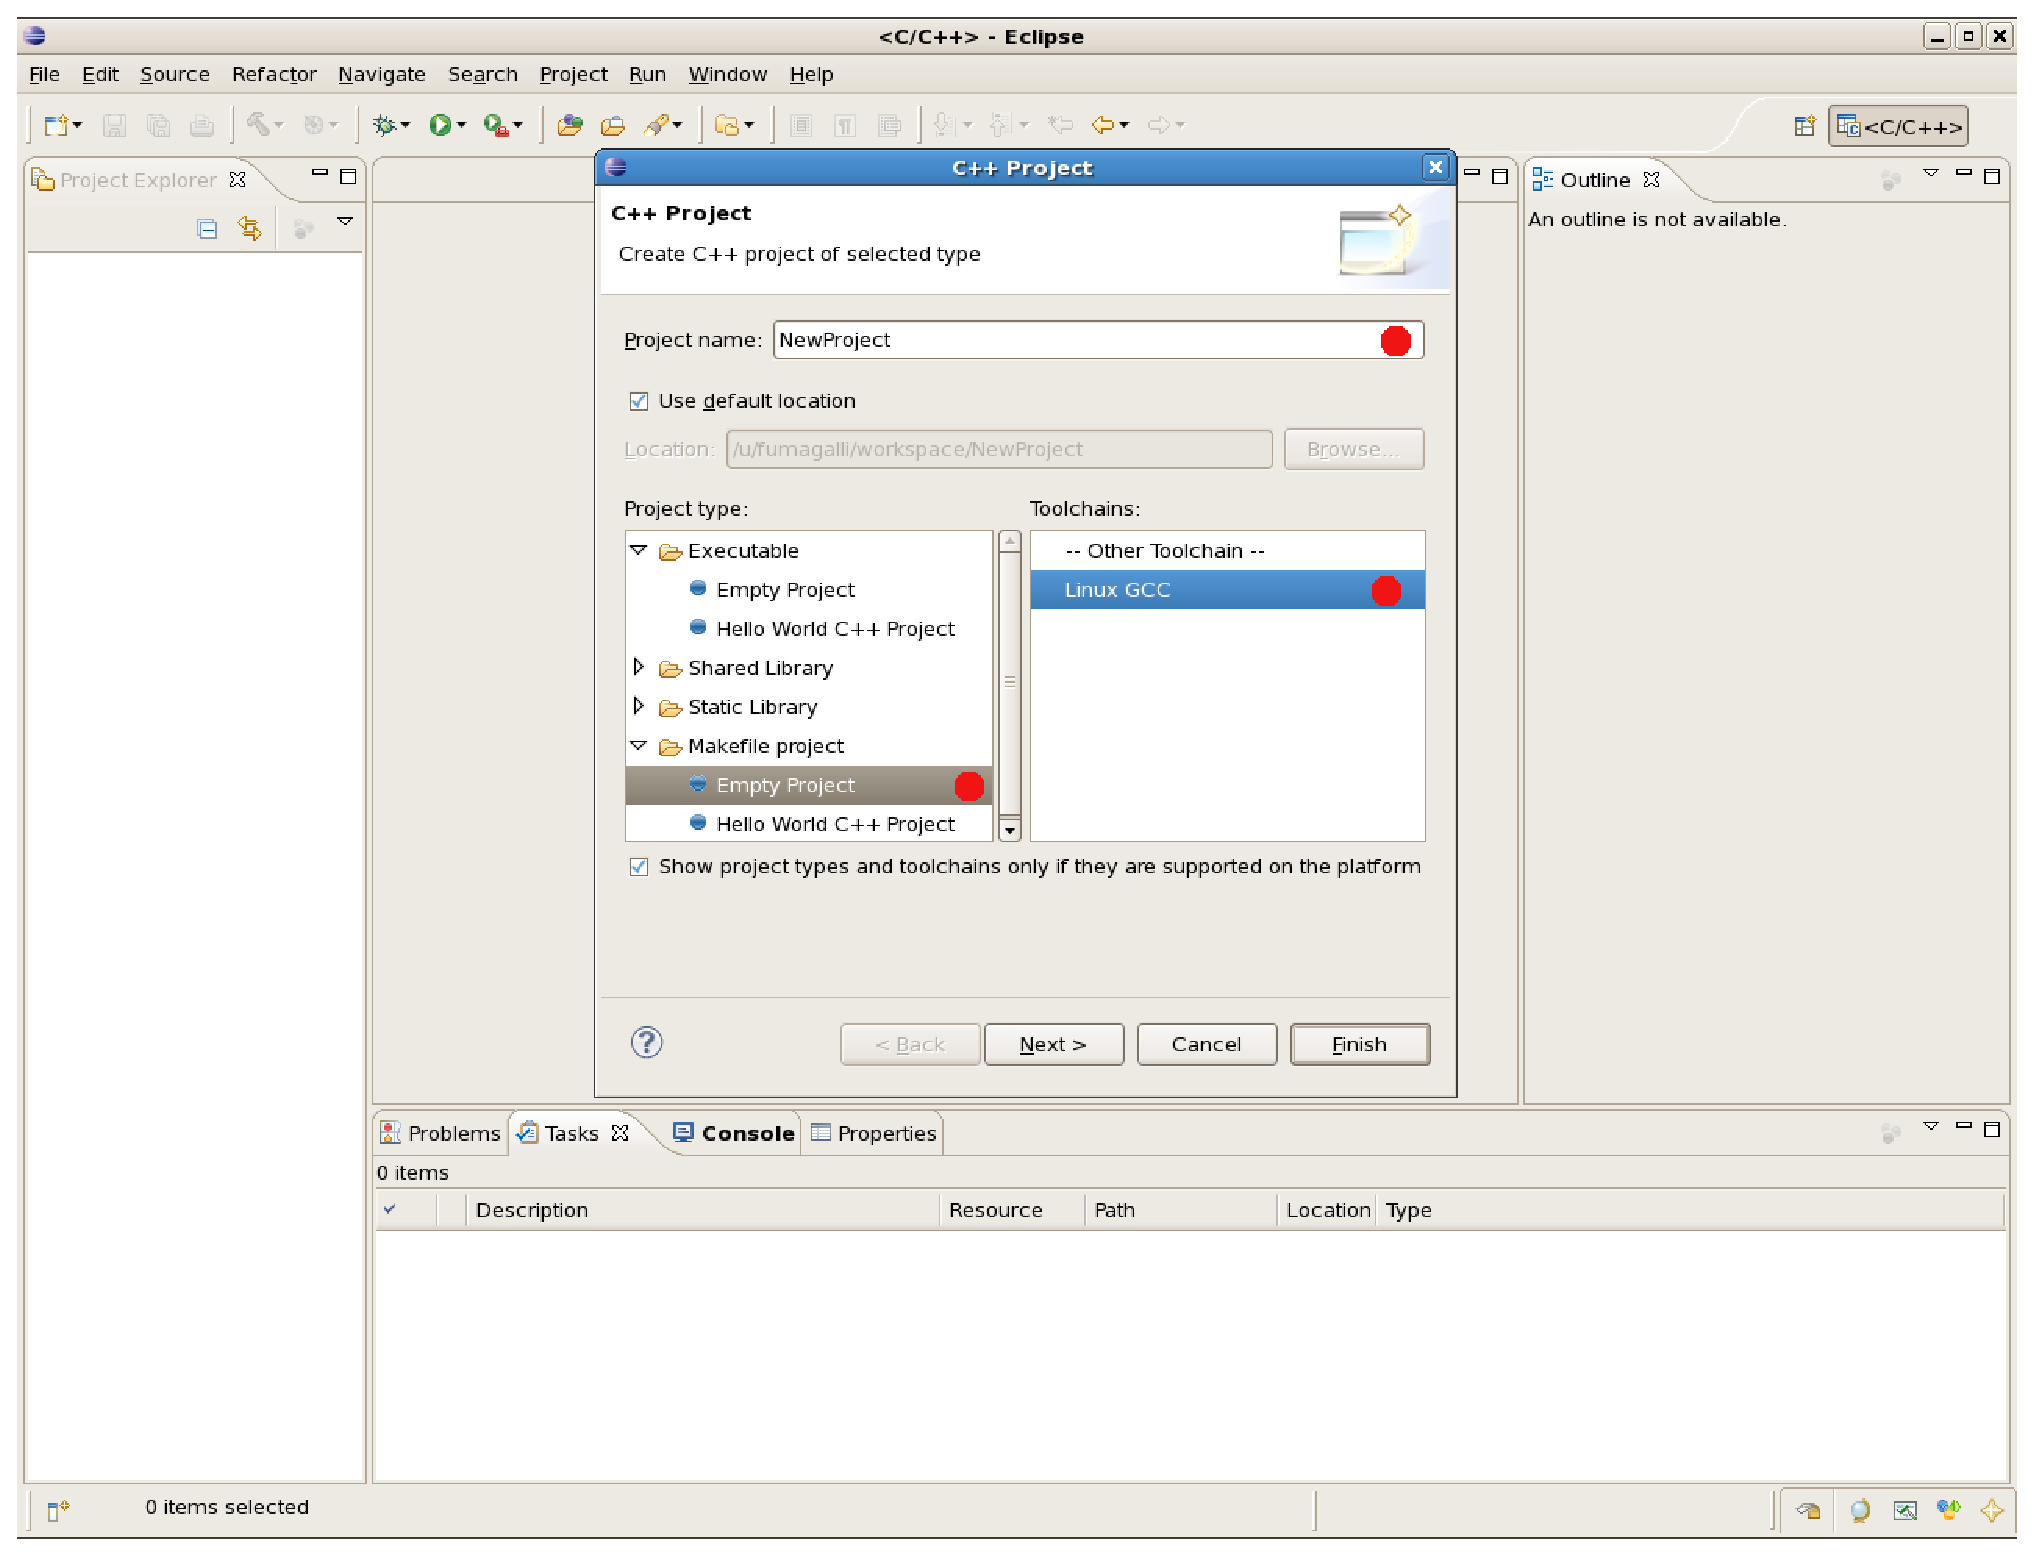
\includegraphics[width=0.95\textwidth]{./images/eclipse2}
    \end{figure}

\end{frame}

%---------------------------------------------------------------------------------

\begin{frame}[fragile]

    \frametitle{Eclipse: insert a cpp file}

    \begin{figure}
        \centering
        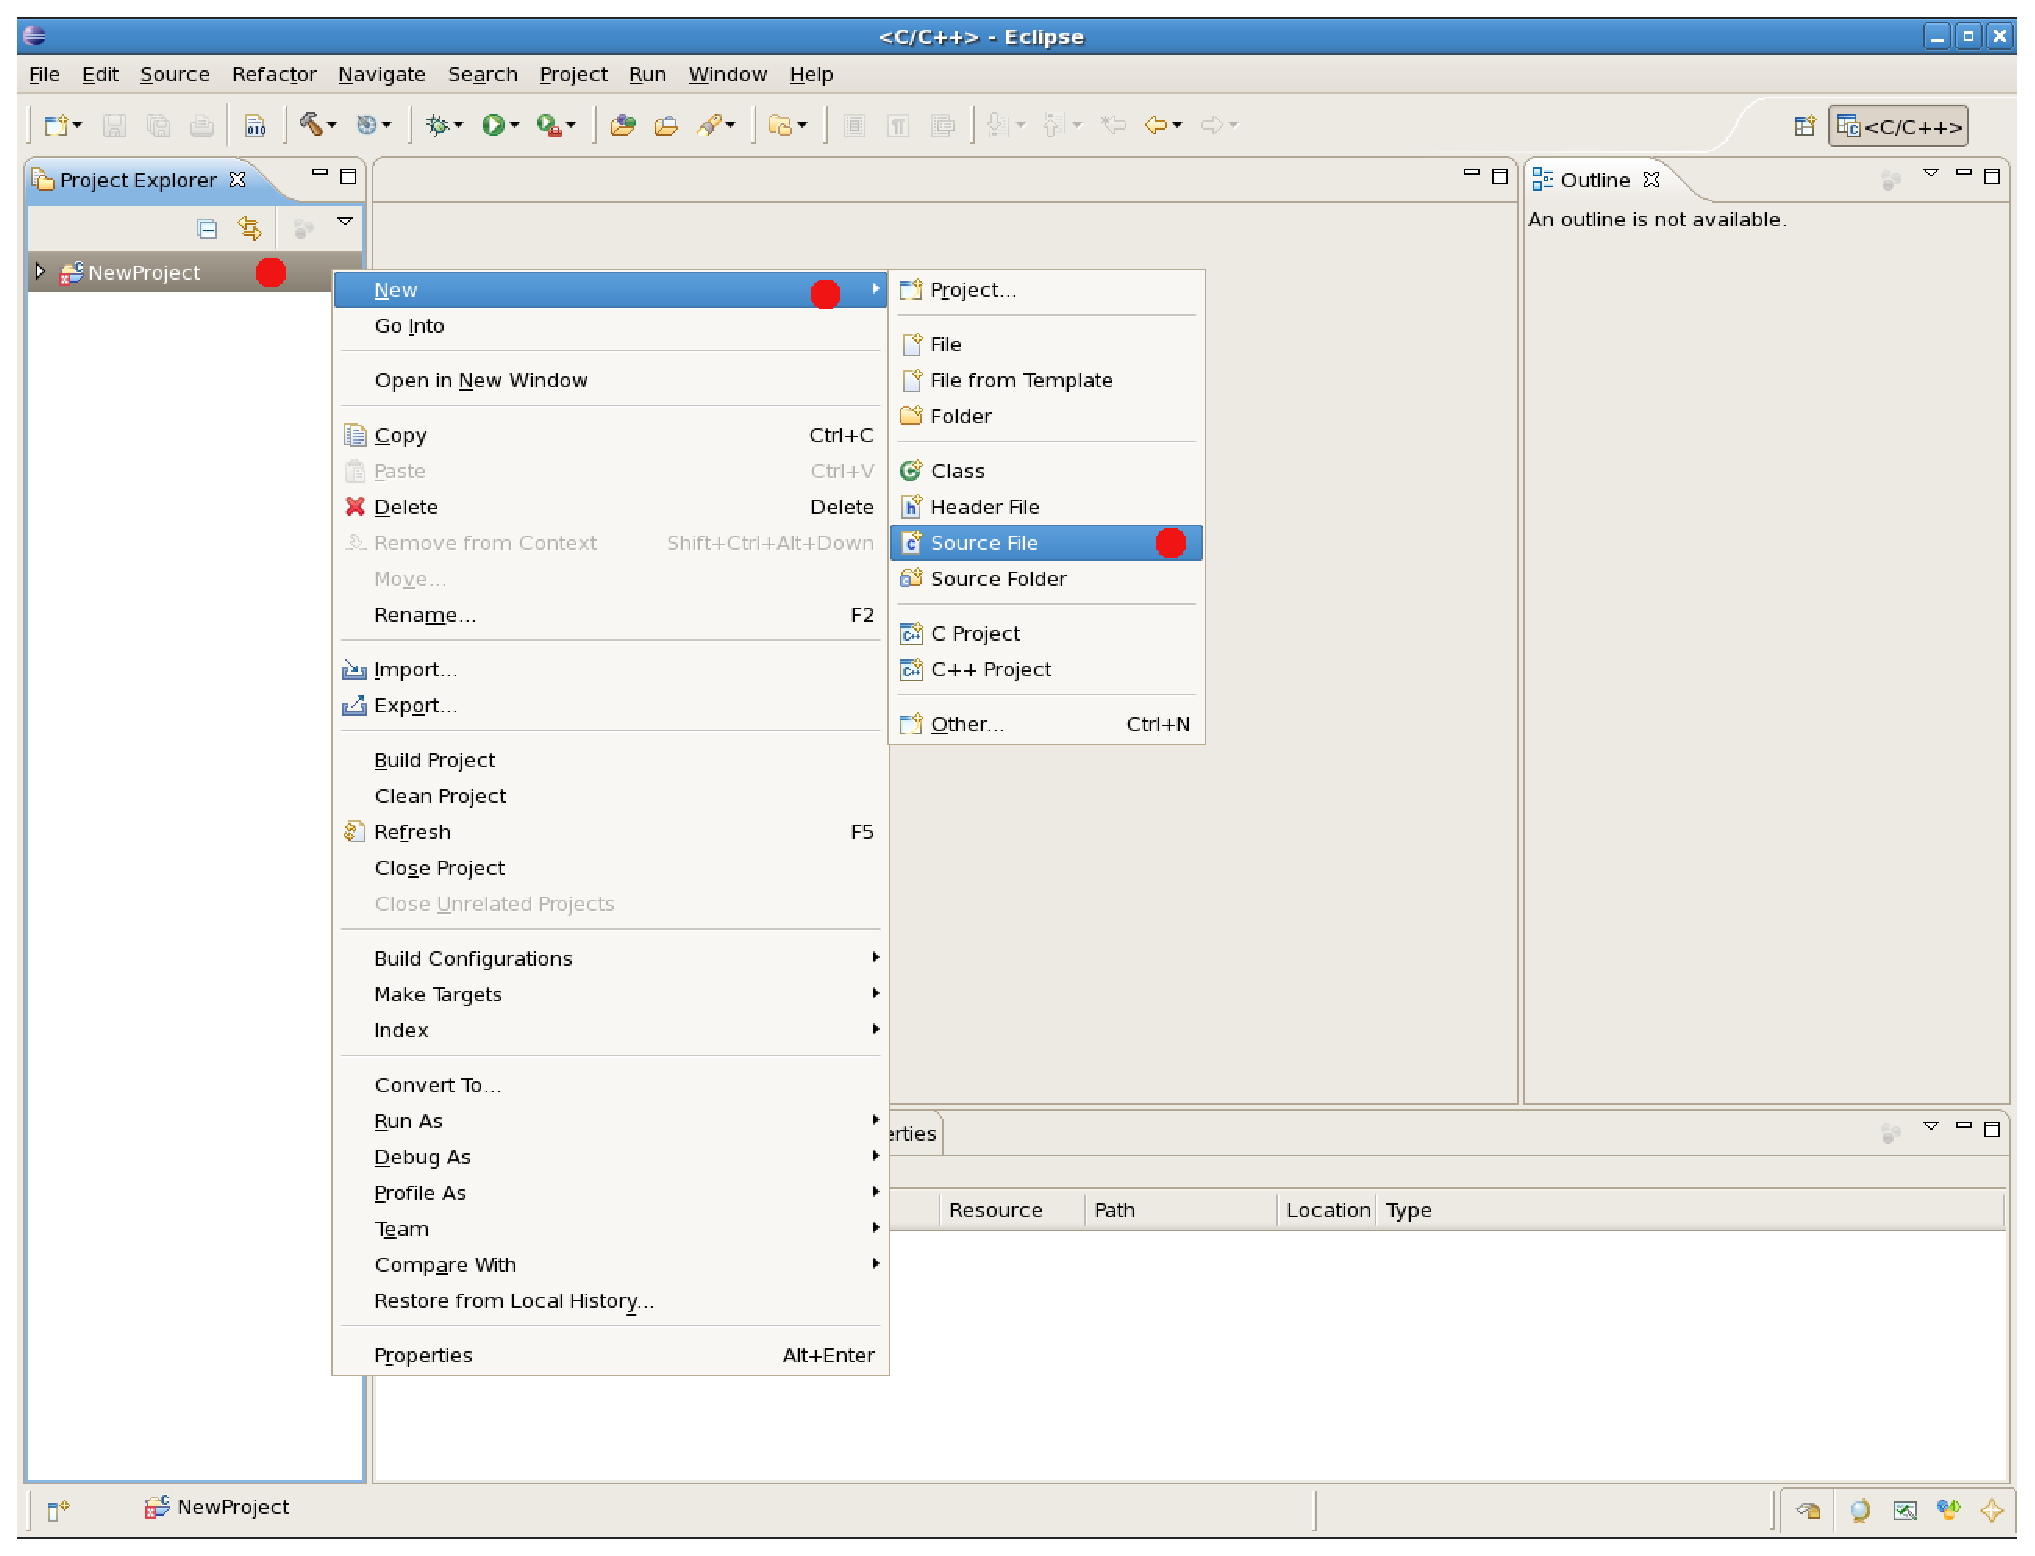
\includegraphics[width=0.95\textwidth]{./images/eclipse3}
    \end{figure}

\end{frame}

%---------------------------------------------------------------------------------

\begin{frame}[fragile]

    \frametitle{Eclipse: insert the name of the source file}

    \begin{figure}
        \centering
        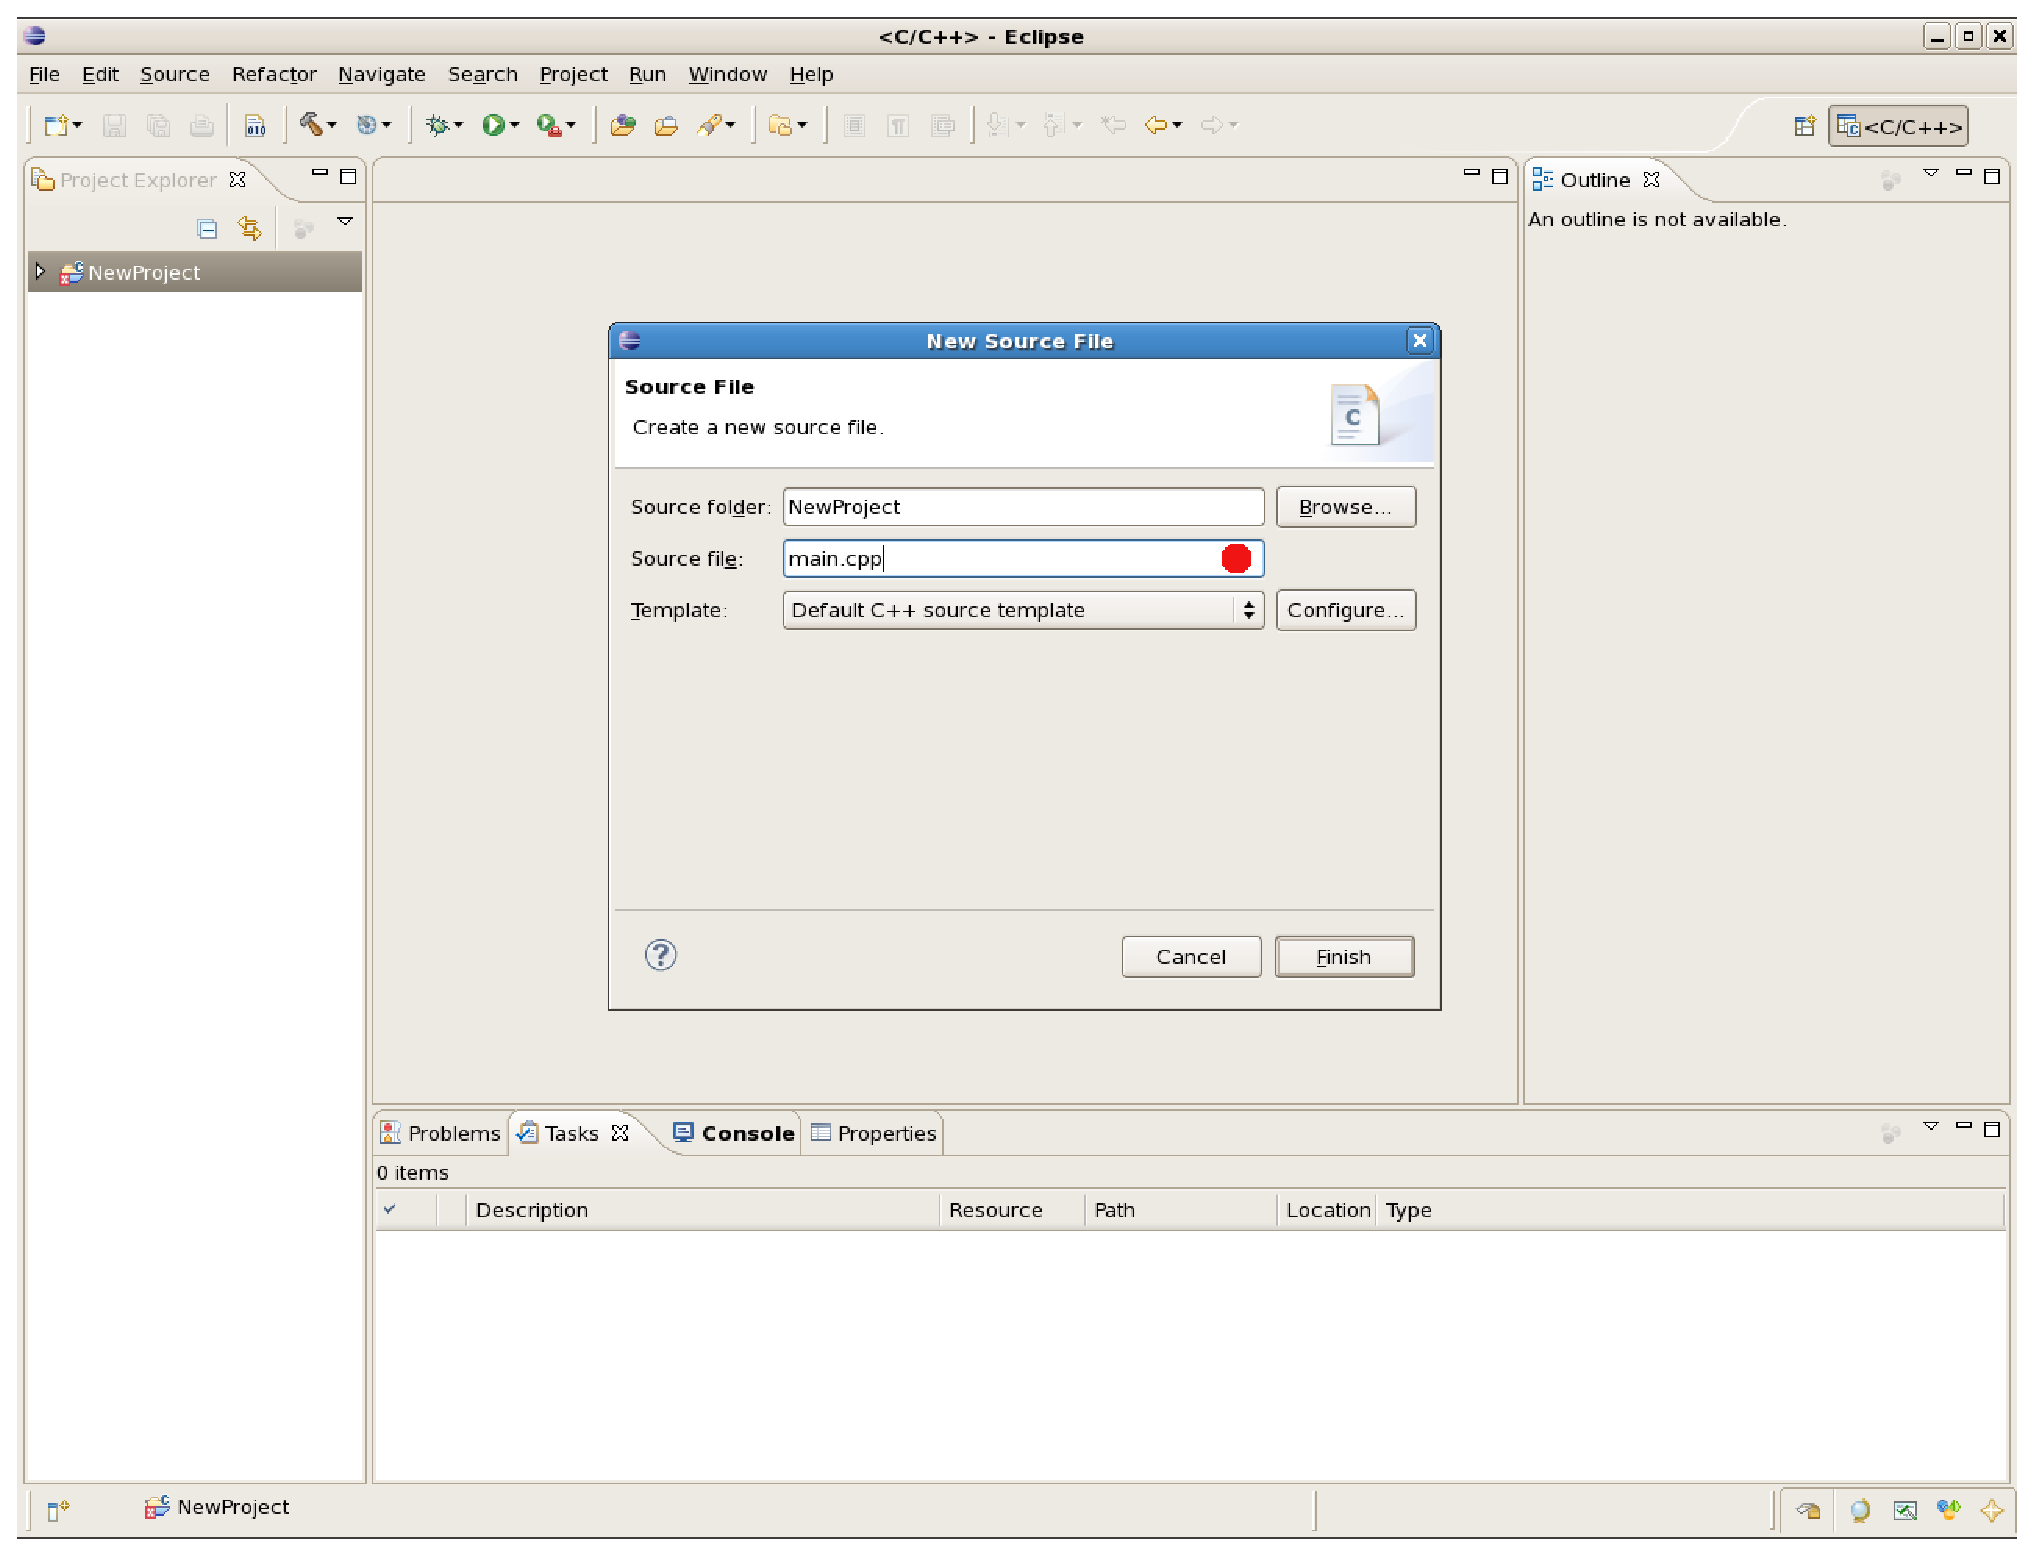
\includegraphics[width=0.95\textwidth]{./images/eclipse4}
    \end{figure}

\end{frame}

%---------------------------------------------------------------------------------

\begin{frame}[fragile]

    \frametitle{Eclipse: example program}

    \begin{figure}
        \centering
        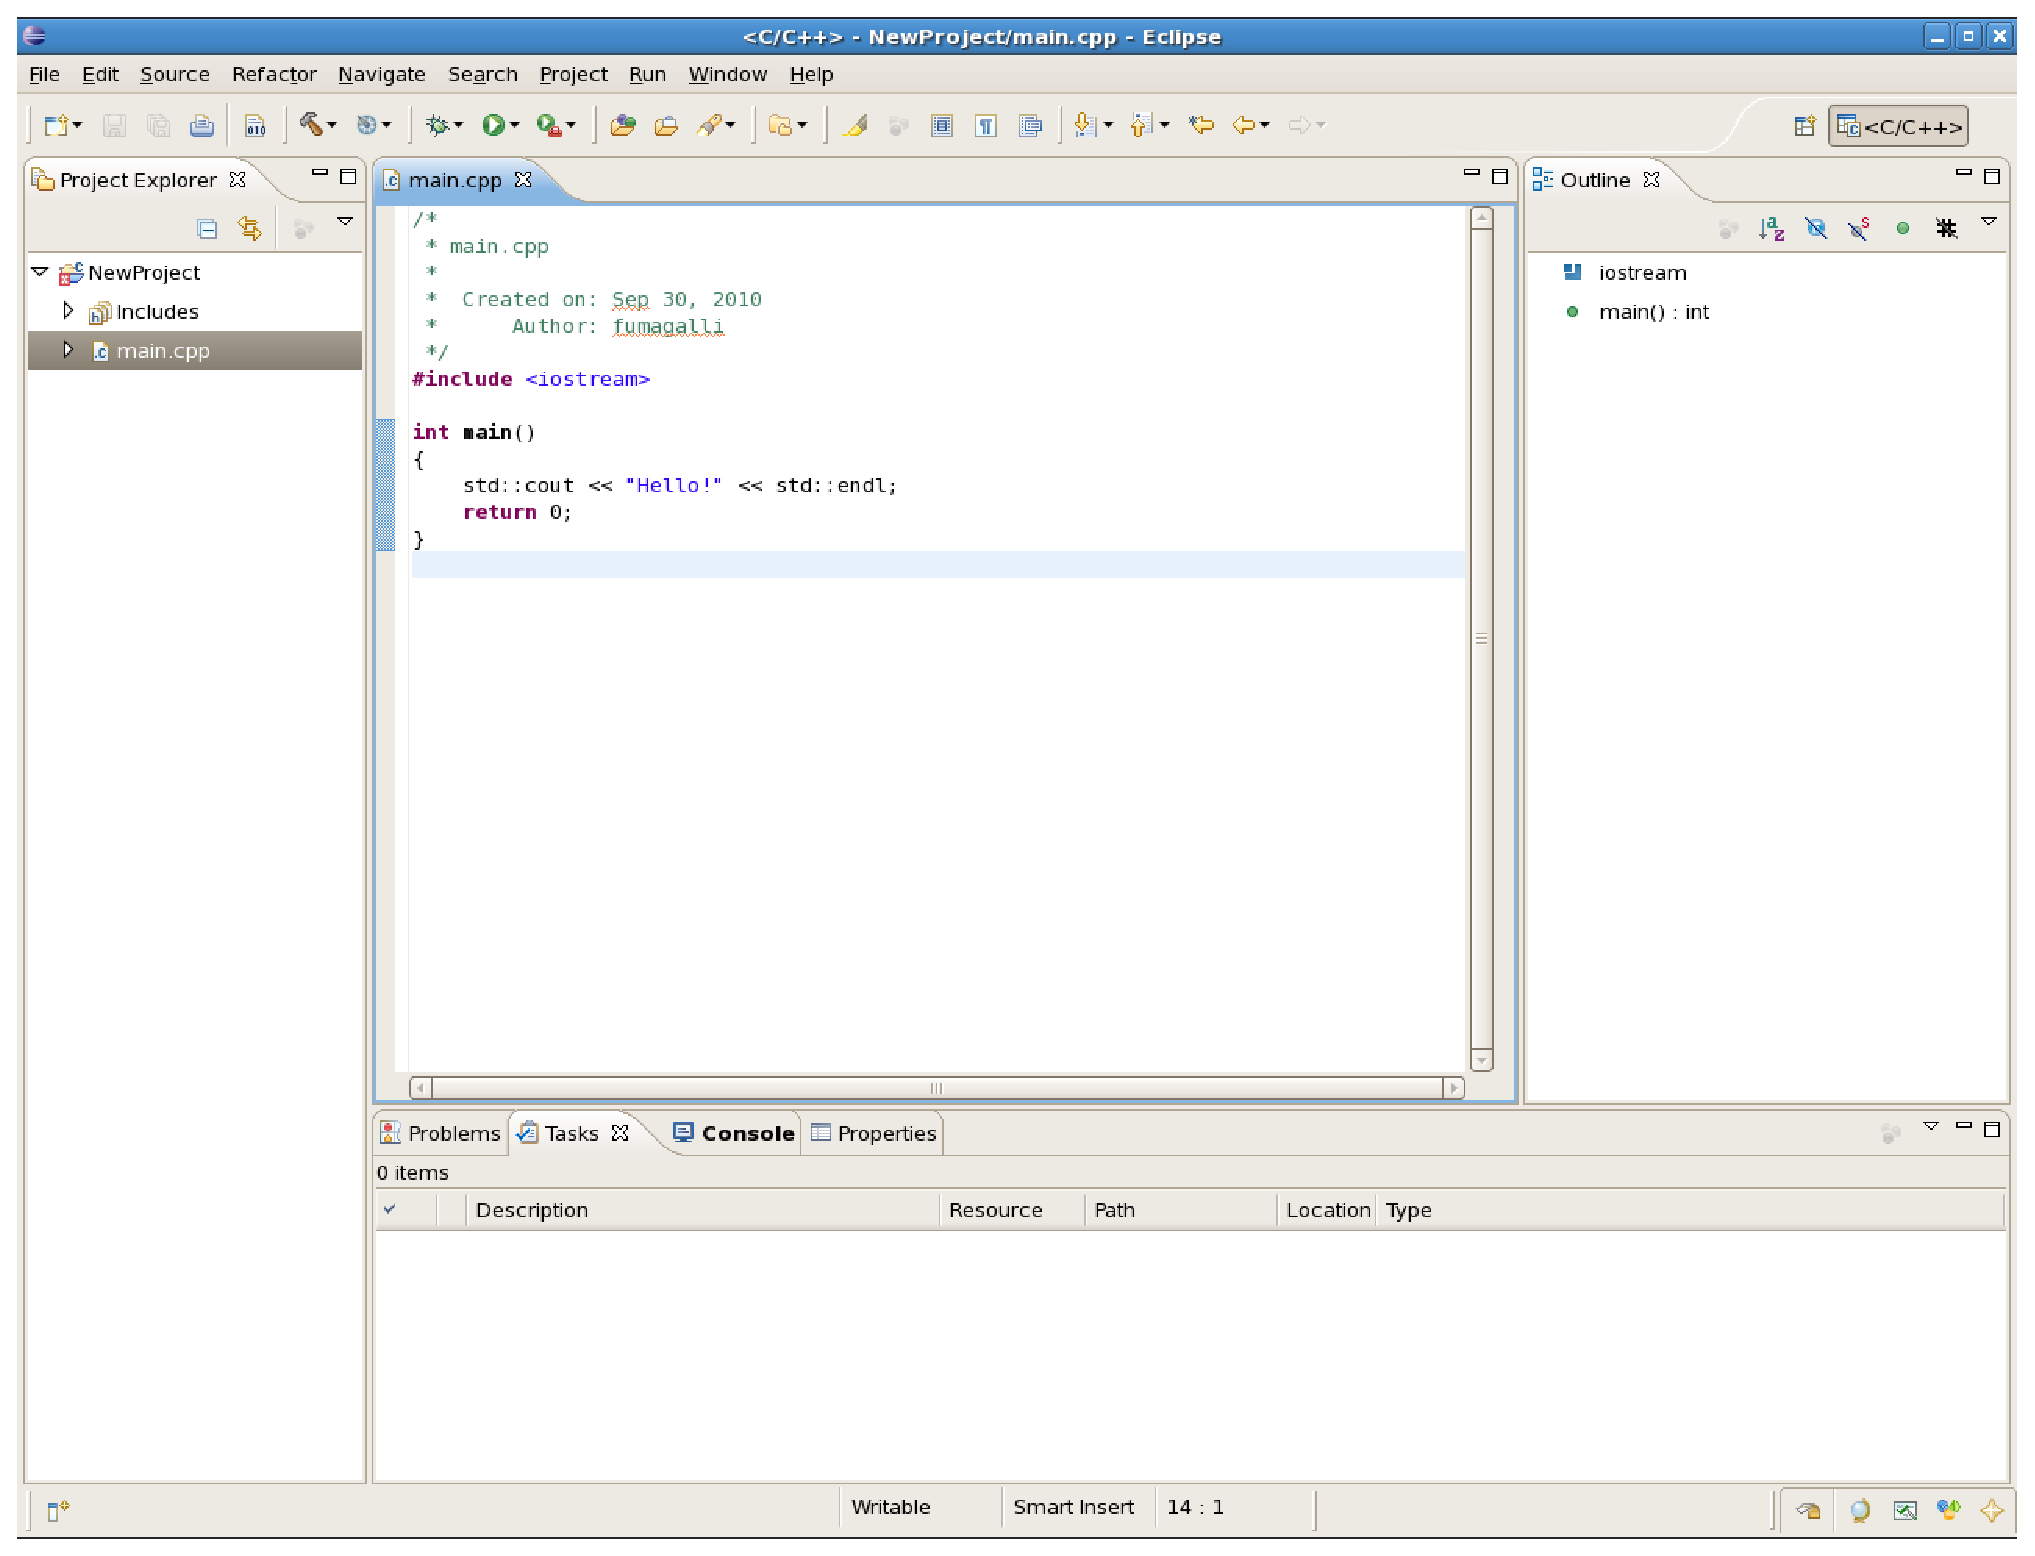
\includegraphics[width=0.95\textwidth]{./images/eclipse5}
    \end{figure}

\end{frame}

%---------------------------------------------------------------------------------

\begin{frame}[fragile]

    \frametitle{Eclipse: to compile we need a Makefile}

    \begin{figure}
        \centering
        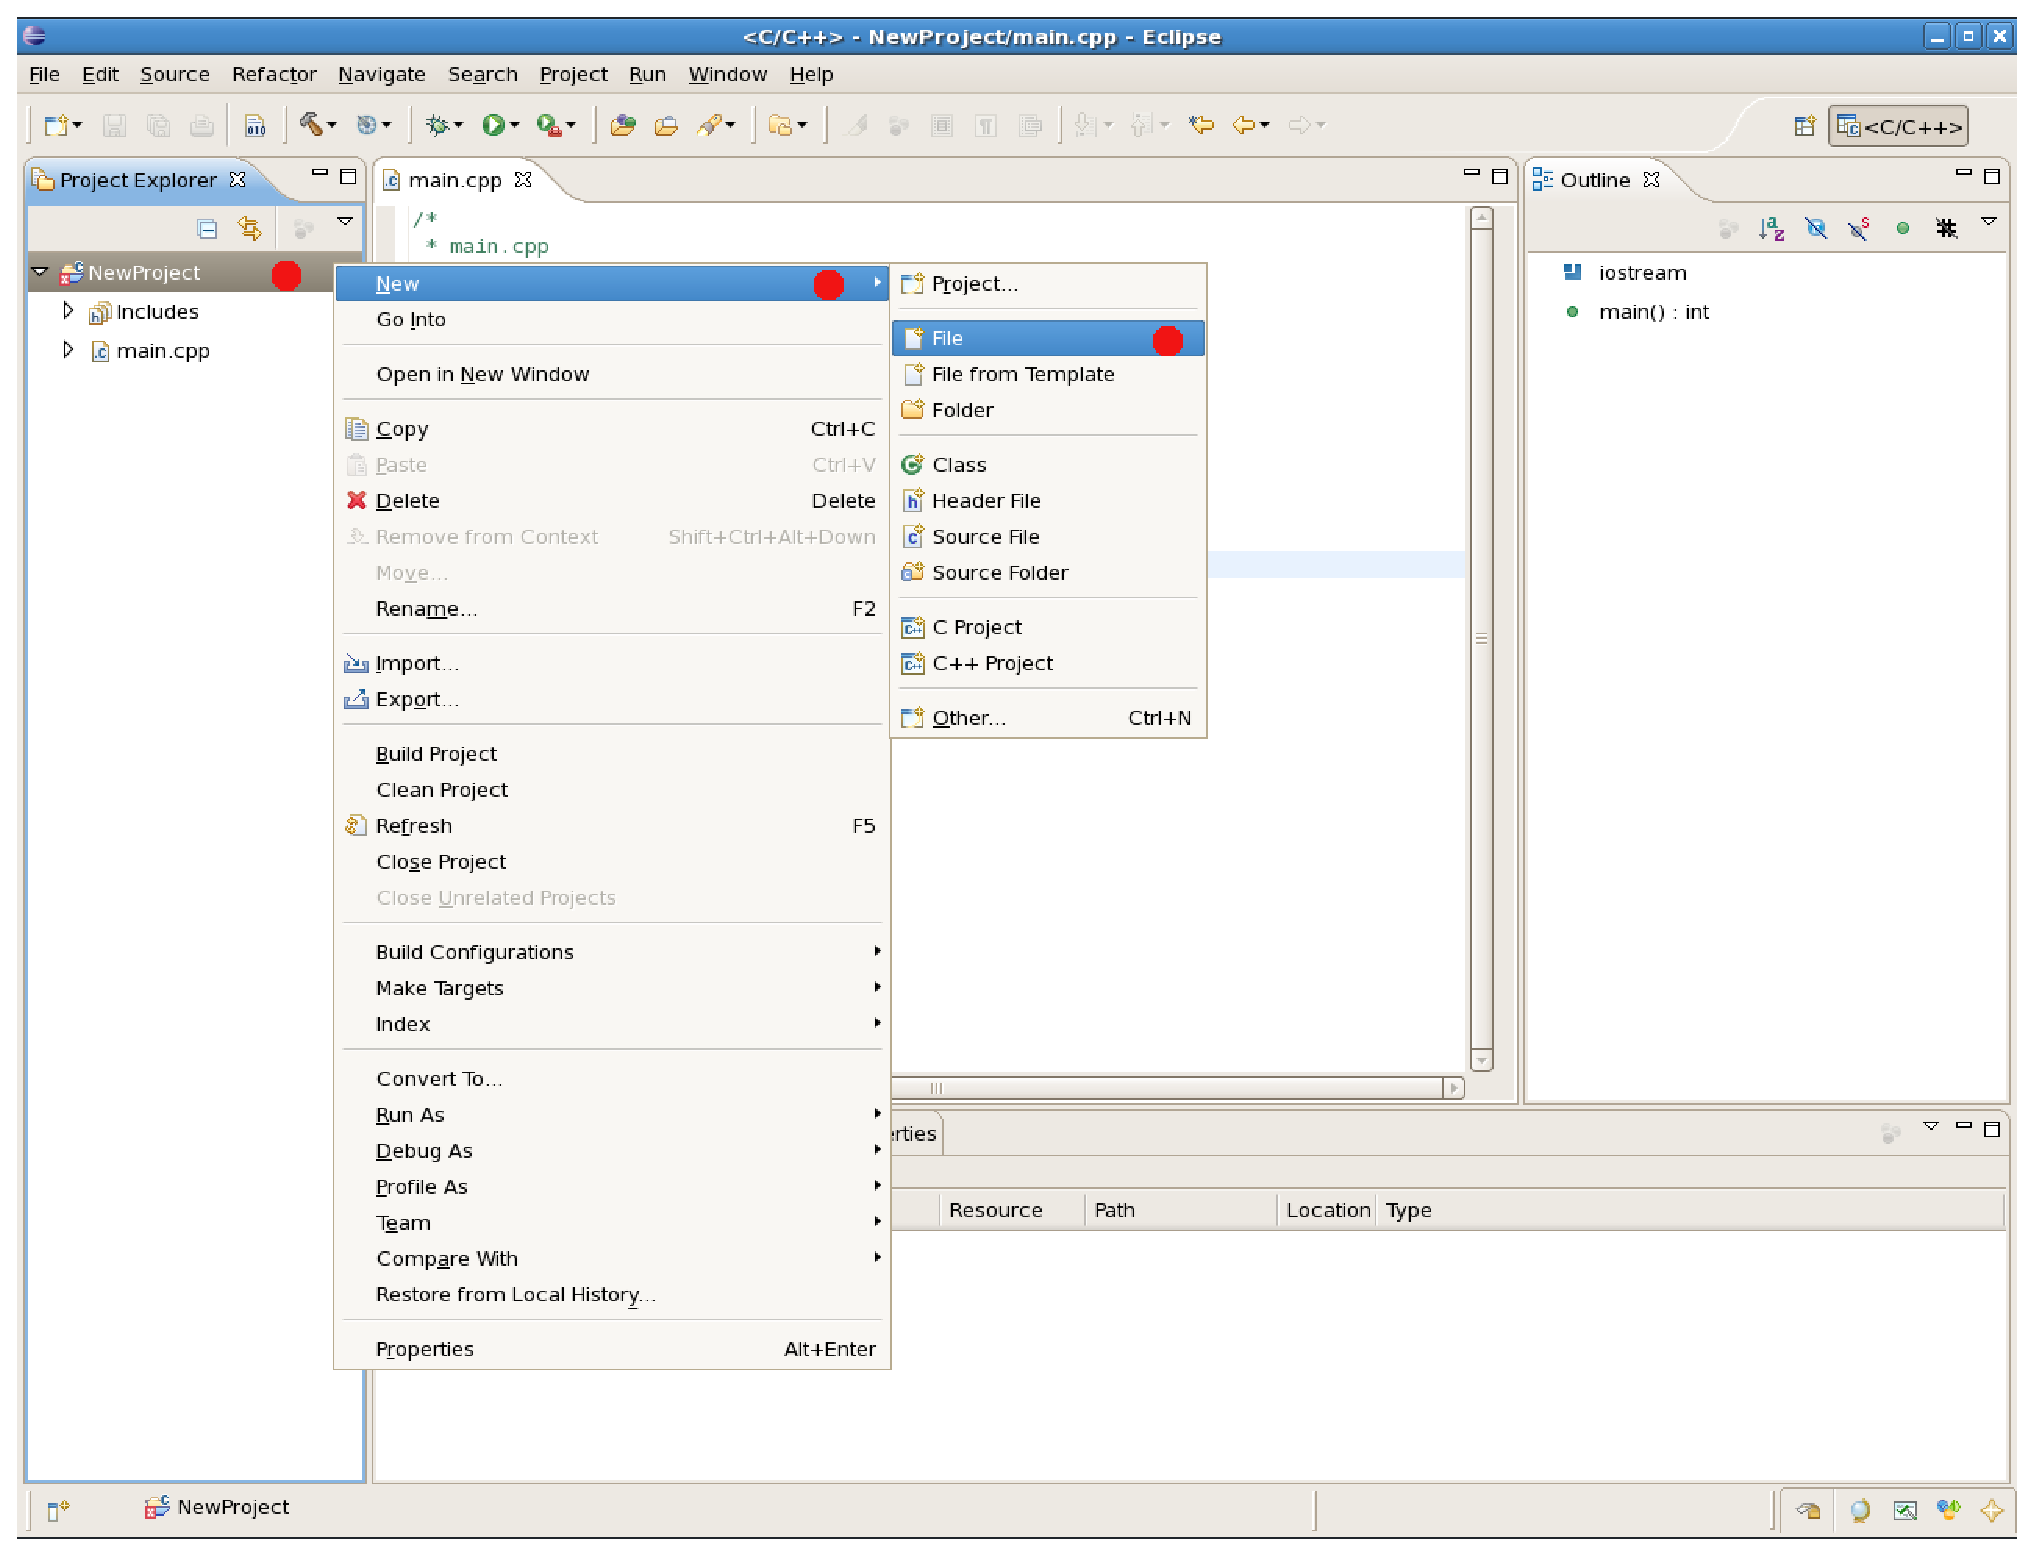
\includegraphics[width=0.95\textwidth]{./images/eclipse6}
    \end{figure}

\end{frame}

%---------------------------------------------------------------------------------

\begin{frame}[fragile]

    \frametitle{Eclipse: insert the name}

    \begin{figure}
        \centering
        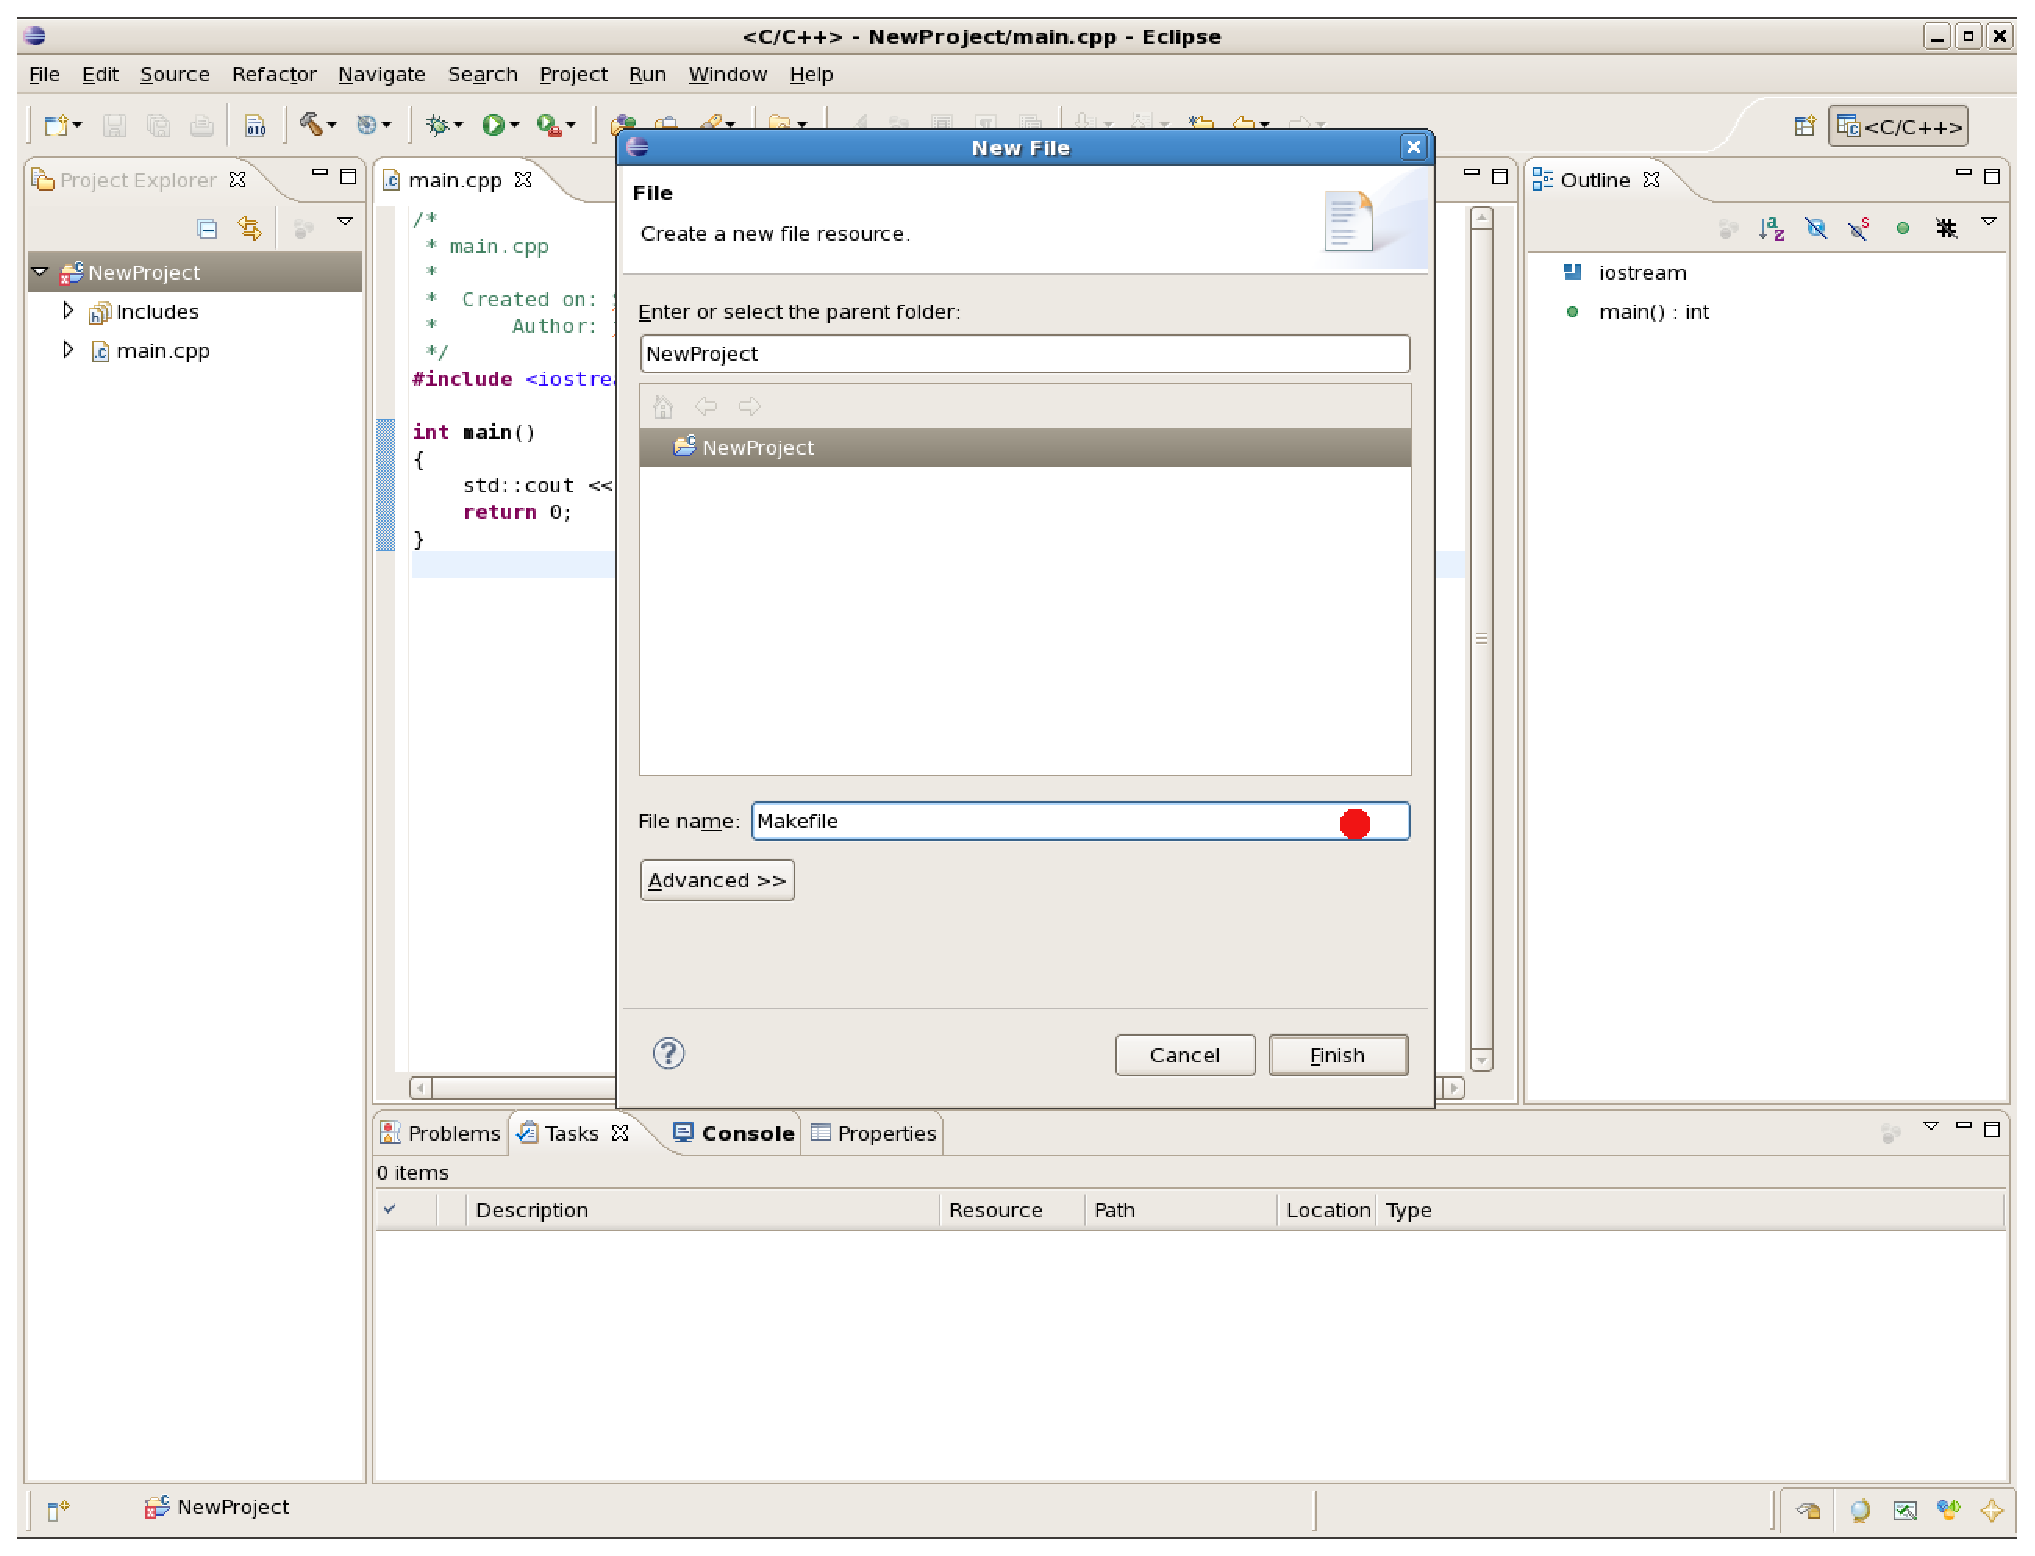
\includegraphics[width=0.95\textwidth]{./images/eclipse7}
    \end{figure}

\end{frame}

%---------------------------------------------------------------------------------

\begin{frame}[fragile]

    \frametitle{Eclipse: write the Makefile}

    \begin{figure}
        \centering
        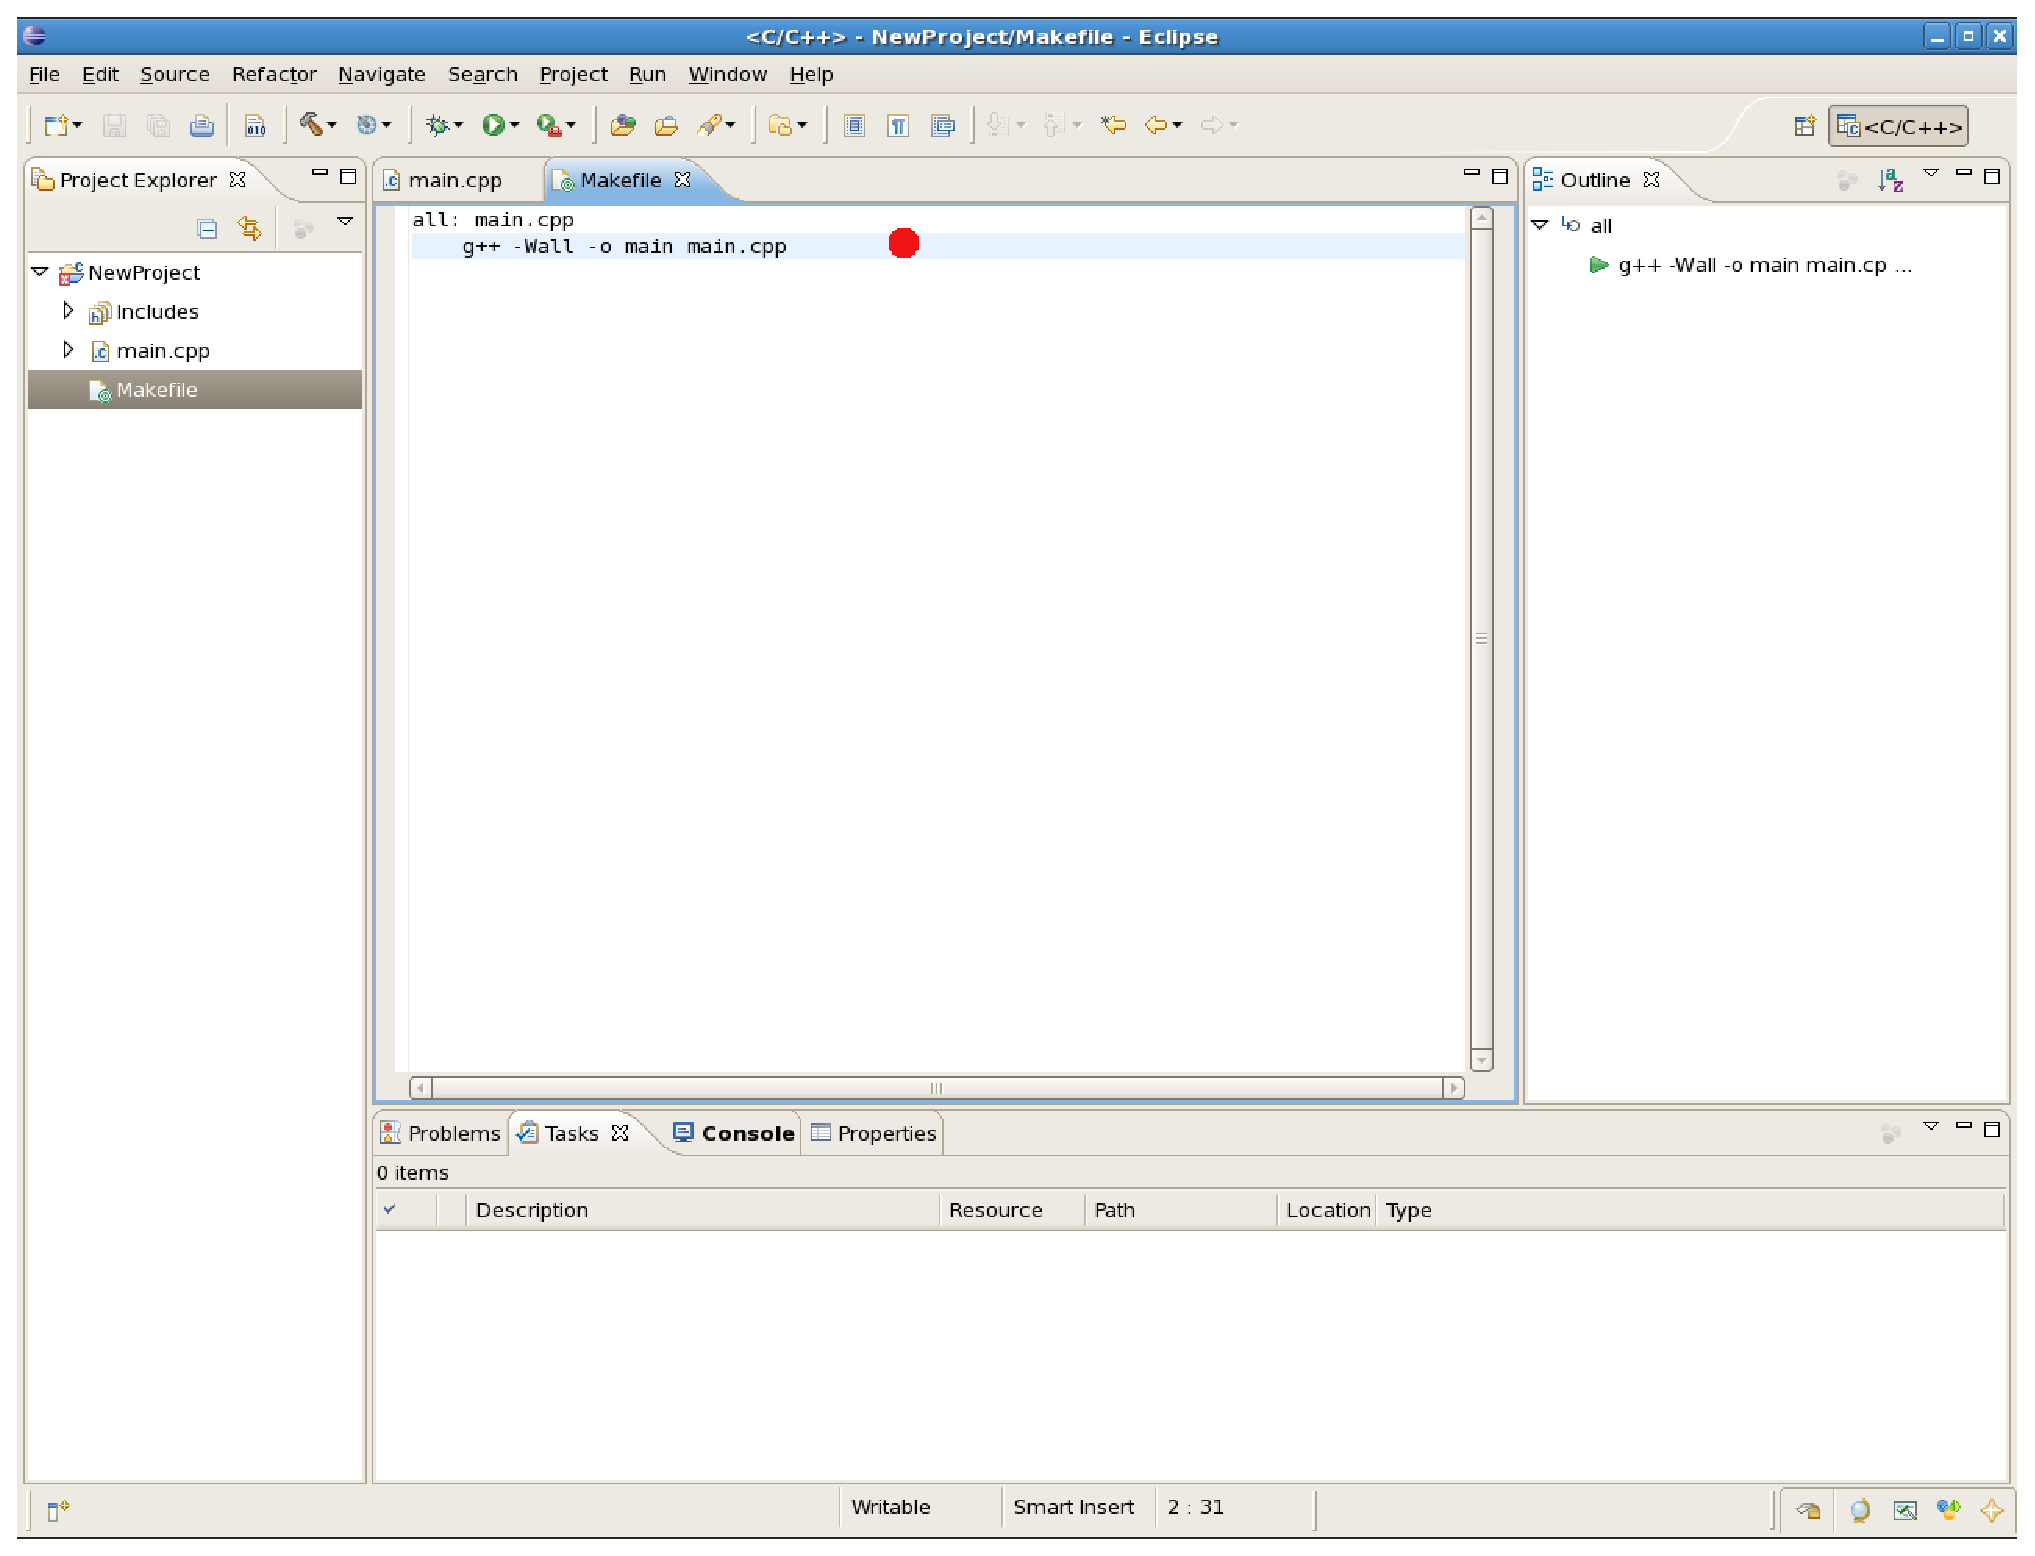
\includegraphics[width=0.95\textwidth]{./images/eclipse8}
    \end{figure}

\end{frame}

%---------------------------------------------------------------------------------

\begin{frame}[fragile]

    \frametitle{Eclipse: set up compilation}

    \begin{figure}
        \centering
        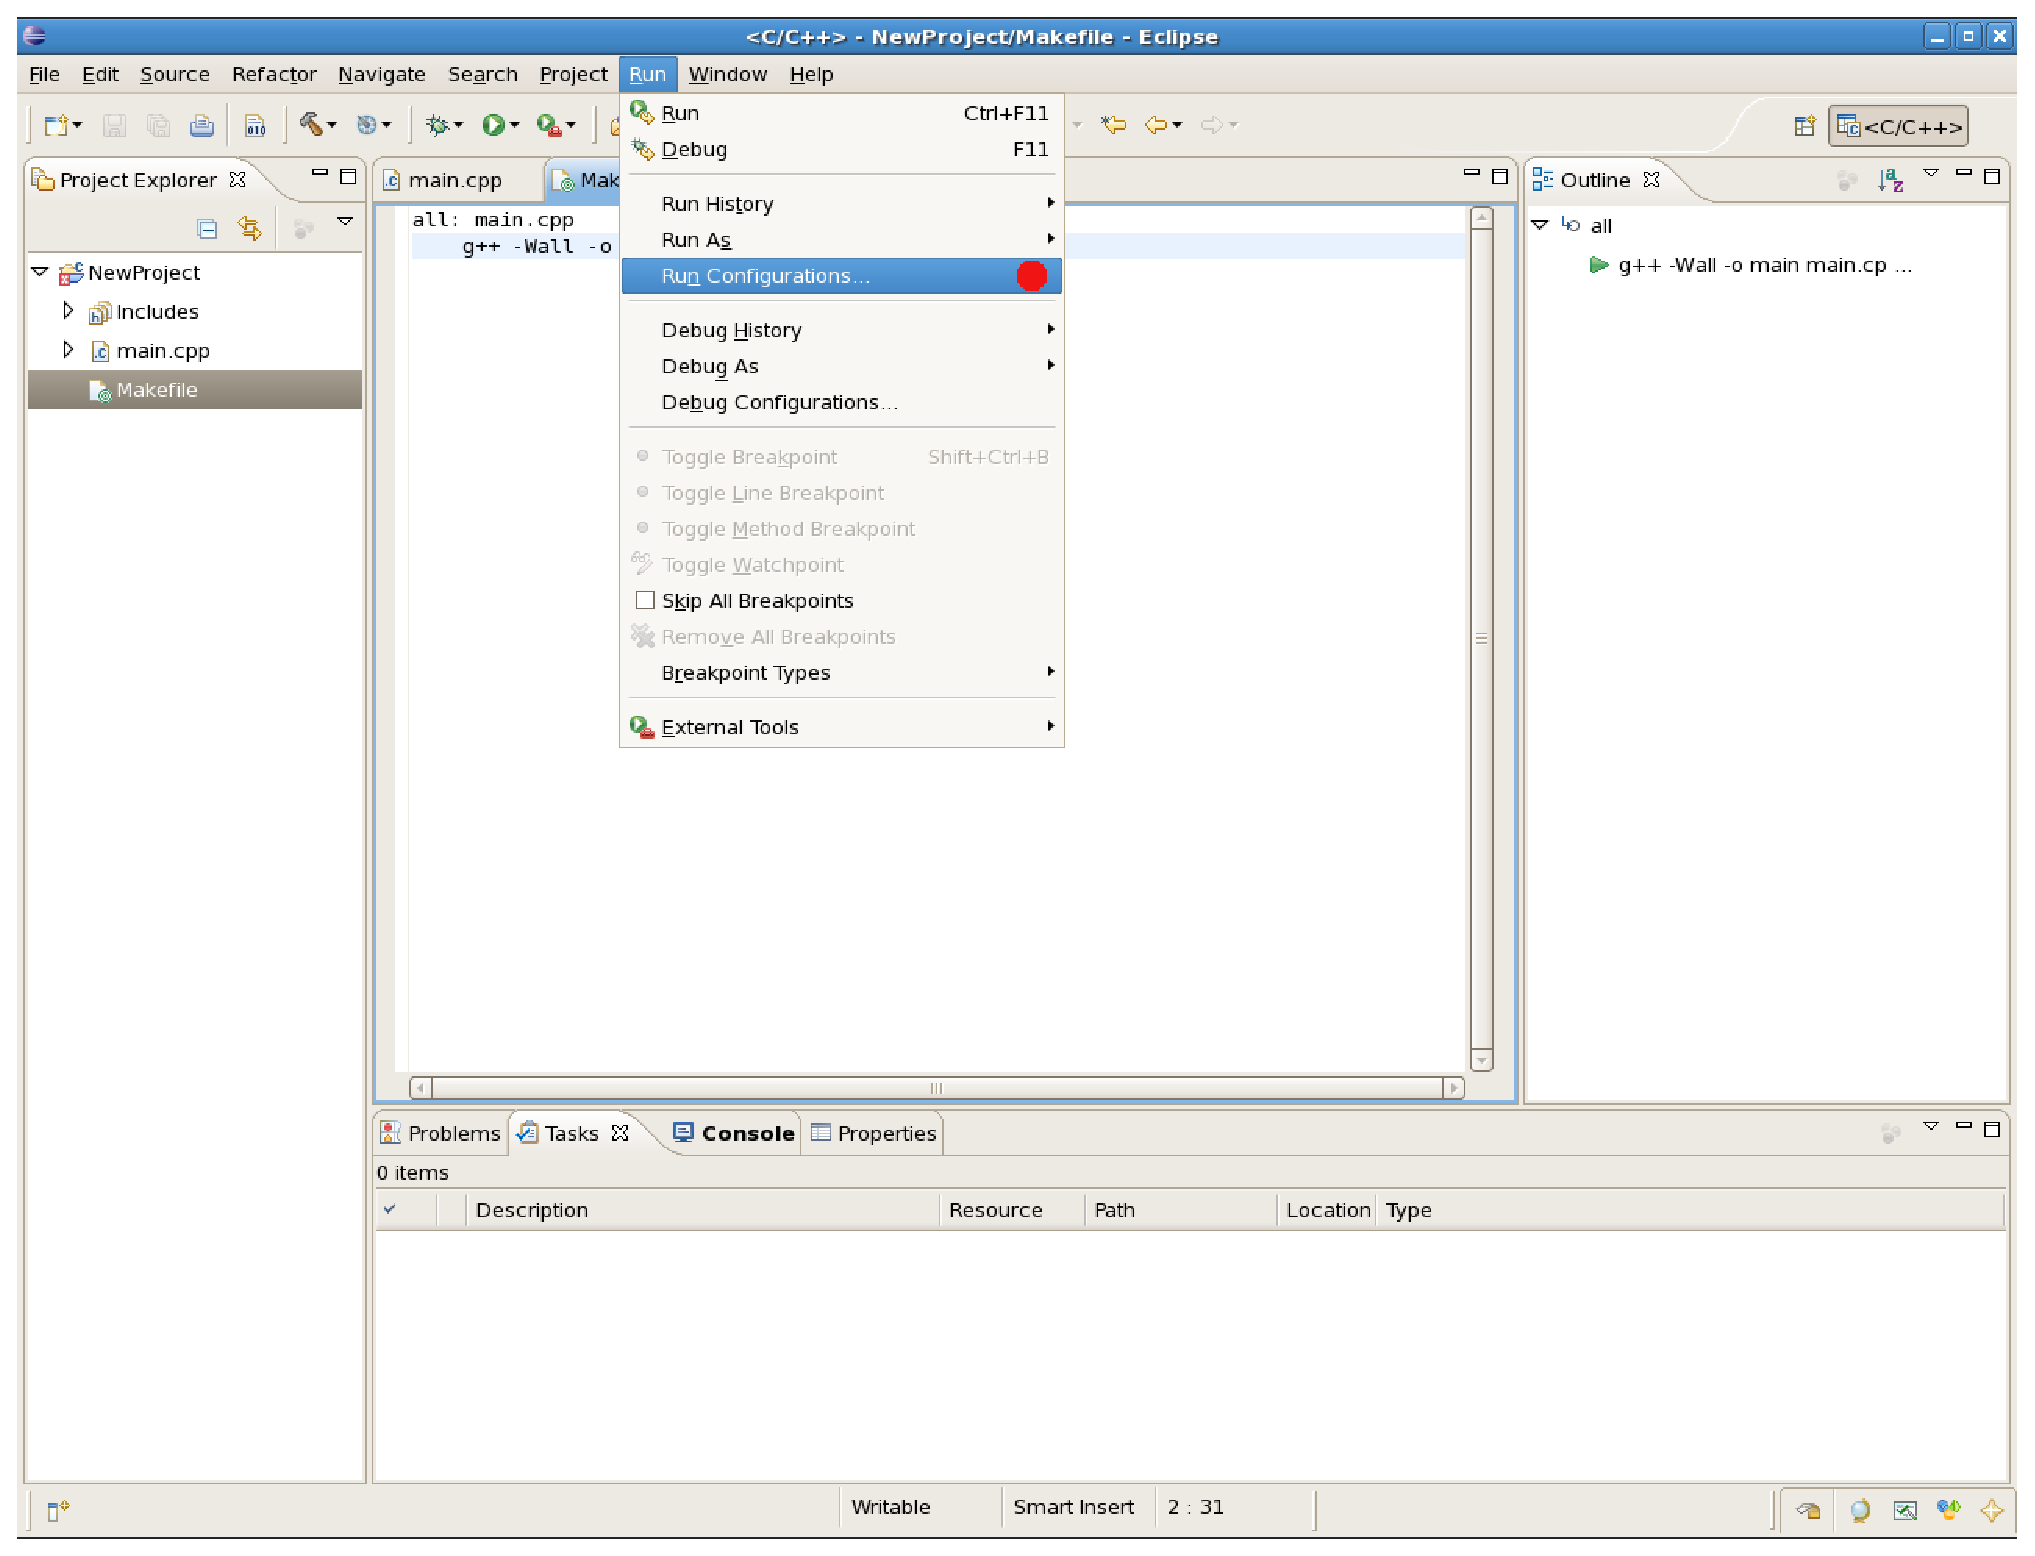
\includegraphics[width=0.95\textwidth]{./images/eclipse9}
    \end{figure}

\end{frame}

%---------------------------------------------------------------------------------

\begin{frame}[fragile]

    \frametitle{Eclipse: set the executable name}

    \begin{figure}
        \centering
        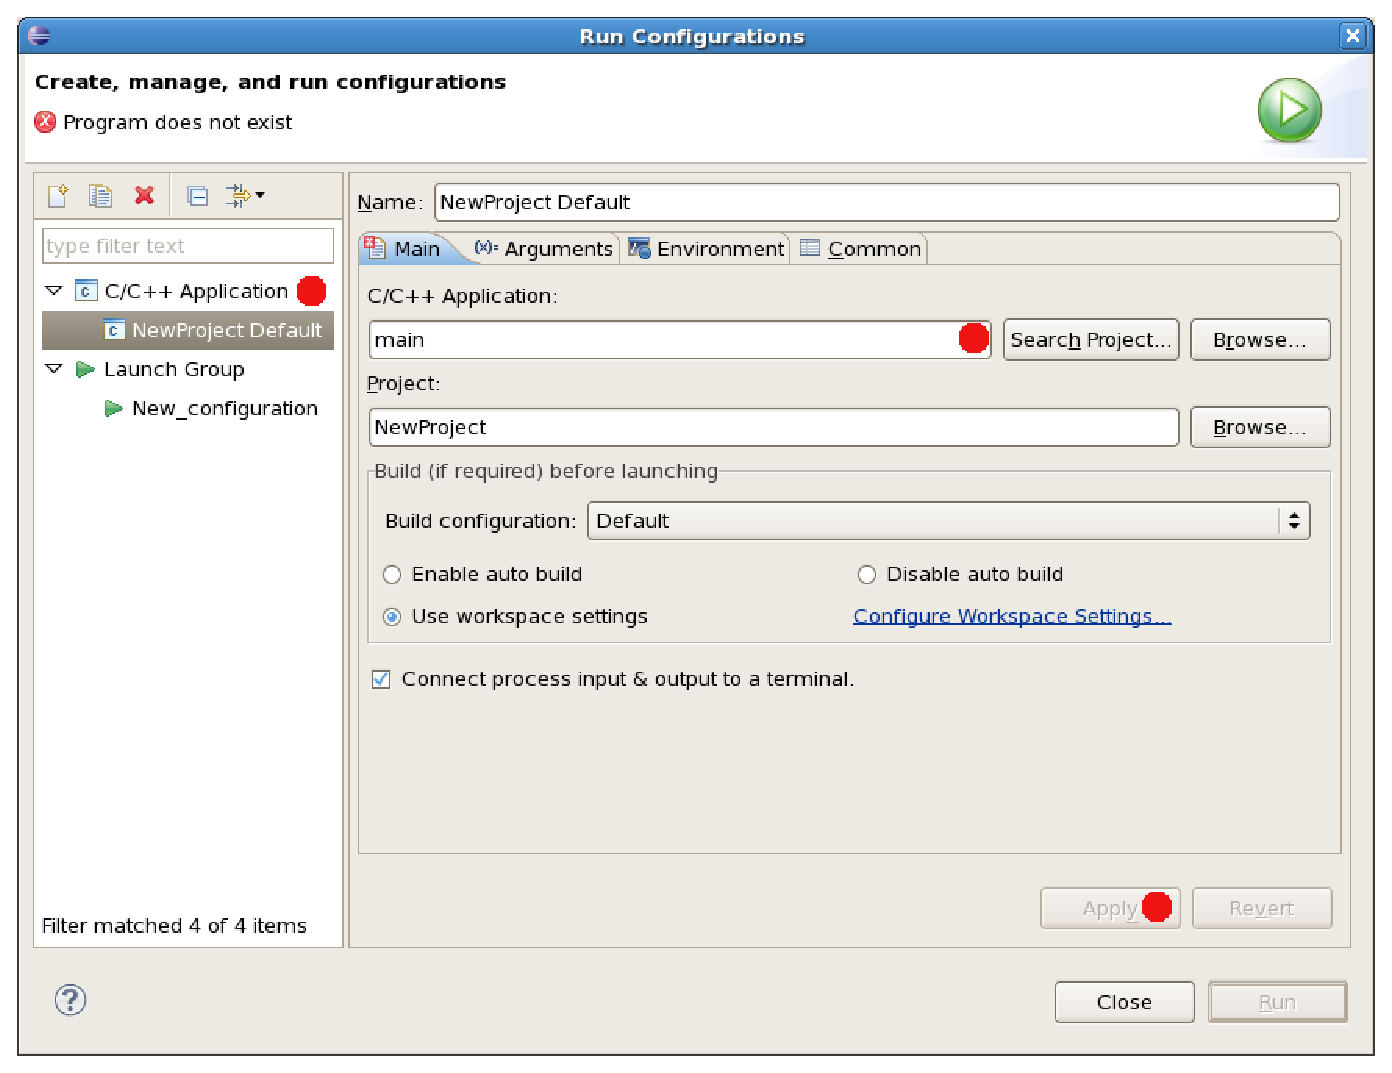
\includegraphics[width=0.95\textwidth]{./images/eclipse10}
    \end{figure}

\end{frame}

%---------------------------------------------------------------------------------

\begin{frame}[fragile]

    \frametitle{Eclipse: compile and execute the program}

    \begin{figure}
        \centering
        \includegraphics[width=0.95\textwidth]{./images/eclipse11}
    \end{figure}

\end{frame}

\end{document}
